\section{Question 3.8}

\subsection{Question}
Suppose that, in an effort to crawl web pages faster, you set up two crawling machines with different starting seed URLs. Is this an effective strategy for distributed crawling? Why or why not?

\subsection{Resources}
The textbook \textit{Search Engines: Information Retrieval in Practice} \cite{seirip}, \textit{Parallel Crawlers} \cite{Cho:2002:PC:511446.511464}, and \textit{Efficient URL Caching for World Wide Web Crawling} \cite{Broder:2003:EUC:775152.775247} were used to answer this question.


\subsection{Answer}
I would say that the answer to this question is ``it depends''.  To maximize effectiveness a solid goal for the designers of this system would be to ensure it downloads each unique page once and only once, minimizing overlap.  Overlap is when a parallel crawler downloads the same page more than once.  This issue can be a problem if there is no communication among the crawling processes and if there are system limitations that cannot be overcome, such as limited bandwidth, maximum hard disk space, or time constraints.  In one of these scenarios overlap can be a debilitating problem, wasting precious resources on repeatedly downloading duplicate web pages.

In order to address the overlap issue, each crawling process would need a way to identify which URLs belong to it, so that it would not crawl URLs that belong to the other crawling machine.  One way of doing this is by partitioning the web prior to the start of the crawling process.  There are a few ways to go about this.  First, the crawlers could receive a static set of seed URLs to start from and then go from there.  This is the simplest route, and is also the one employed by Cho and Garcia-Molina in \cite{Cho:2002:PC:511446.511464}.  Another method is to use a central controller to divide the web into partitions and then, as these URLs are discovered by the crawling processes, the central controller sends them to the responsible crawling process.  If this issue is not addressed by the parallel crawling machines then overlap will become a problem.

In addition to the partitioning scheme, the two crawlers would benefit from using some inter-process communication to inform each other which URLs have been visited, which mitigates the overlap issue described above.  This communication would cause some additional processing and network bandwidth consumption, but can be minimized by using batched dispatching \cite{Cho:2002:PC:511446.511464} and a URL caching scheme \cite{Broder:2003:EUC:775152.775247}.

Another issue for parallel crawlers is coverage.  Coverage is how much of the web is downloaded.  If the crawler is downloading pages to build an index for a search engine coverage can be an important issue.  If the crawlers do not cooperate with each other coverage can suffer under certain circumstances.  For example, in Figure \ref{fig:cproc}, \(S_1\) is a partition of websites assigned to Crawler \(C_1\), and \(S_2\) is a partition of websites assigned to Crawler \(C_2\).  If the crawlers do not communicate with each other and also do not traverse the inter-partition links, Crawler \(C_1\) will not discover pages \(d\) or \(e\), and so coverage will suffer.  If coverage is important then the parallel crawling machines should pass URLs to each other to minimize the pages missed due to these limitations.

These are but a few items to ponder when going about designing a parallel crawler.  They can be effective at their job if they are designed to mitigate these issues, but if they are not addressed then the crawler will likely not be very effective at all.

\clearpage

\begin{figure}[h!]
\centering
\label{fig:cproc}
\fbox{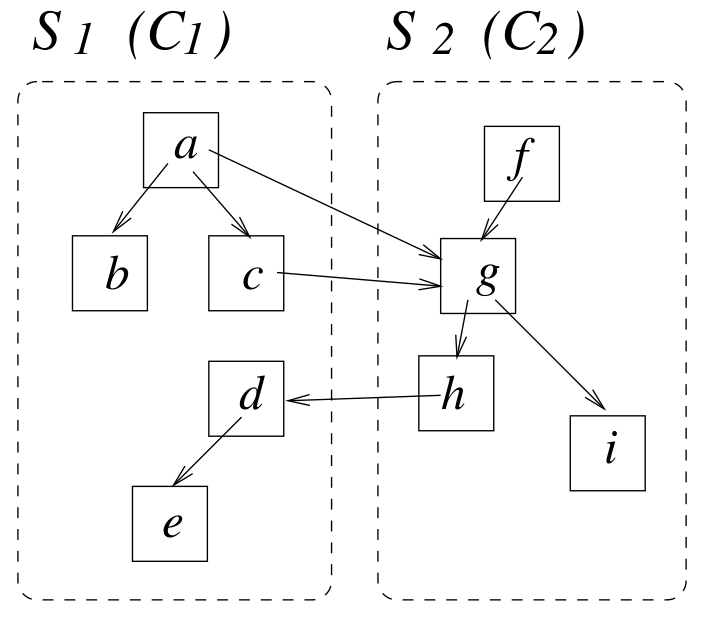
\includegraphics[scale=.5]{q3.8/pc_fig2_cho_garcia-molina.png}}
\caption[Two site example]{Two site example\protect\footnotemark}
\end{figure}

\footnotetext{Source: Junghoo Cho and Hector Garcia-Molina. Parallel Crawlers. In \textit{Proceedings of the 11th International Conference on World Wide Web}, WWW '02, page 126, New York, NY, USA, 2002. ACM.}